\section{Experiments and Results}
\label{sec:experiments}

In this section, we conduct extensive empirical evaluations to validate the proposed multi-platform hybrid framework. The experiments are designed to investigate four core hypotheses:
1) whether the constraint-aware macroscopic planner effectively prevents fluid spillage;
2) whether the posture-aware massively parallel DRL agent guarantees upright labware grasping;
3) whether the regularized few-shot fine-tuning pipeline successfully bridges the sim-to-real gap for IL-based micro-pipetting; and
4) whether the complete system can seamlessly execute the end-to-end bio-chemical assay workflow autonomously.

For binary outcomes with available success and trial counts, 95\% confidence intervals (CIs) are computed using the Wilson score method:
\begin{equation}
    \begin{aligned}
    D &= 1+z^2/n,\quad z=1.96,\\
    c &= (\hat p+z^2/(2n))/D,\\
    h &= \frac{z}{D}\sqrt{\frac{\hat p(1-\hat p)}{n}+\frac{z^2}{4n^2}},\\
    \text{CI}_{95\%} &= [c-h,c+h].
    \end{aligned}
\end{equation}
where $\hat{p}$ is the observed success rate and $n$ is the number of trials.
Continuous outcomes require substrate- or episode-level uncertainty estimates. Significance testing is reserved for comparisons with independent or explicitly paired trial records; percentages alone do not establish significance.

\subsection{Experimental Setup and Hardware Configuration}
\label{subsec:exp_setup}

The physical validation platform strictly mirrors the Isaac Sim simulation setup. The mobile manipulation system features a differential-drive chassis equipped with a 6-DoF UR3 robotic arm. A Robotiq 2F-85 parallel gripper, fitted with custom compliant rubber pads, is used to secure fragile glassware and microplates.

For the perception subsystem, an Intel RealSense D435 RGB-D camera is mounted in an eye-to-hand configuration, providing continuous point cloud and visual feedback. The computational pipeline---encompassing real-time 3D voxel costmap generation, DRL policy inference, and Hierarchical State Machine (HSM) sequencing---is executed locally on an NVIDIA RTX 4090 workstation, ensuring low-latency communication via a ROS bridge.

\subsection{State Synchronization Results}
\label{subsec:state_sync_eval}
Table~\ref{tab:sync_illustrative} reports the measured summary values supplied for the simulation--physical state interface. The reported values meet the specified targets for joint-state agreement, object-pose error, update delay, observation validity, and grasp-state recognition. Object-pose errors should be computed against an independent reference rather than the RGB-D estimate used to update the simulation. The number of runs, raw timestamped trajectories, reference-measurement procedure, and uncertainty intervals were not supplied with these summary values; they remain necessary for independent verification and statistical analysis. The task-success rates reported below evaluate separate tasks and should not be treated as state-synchronization results.

\begin{table}[!t]
\caption{State synchronization targets and reported measured results}
\label{tab:sync_illustrative}
\centering
\resizebox{\columnwidth}{!}{%
\begin{tabular}{lcc}
\hline\hline
\textbf{Metric} & \textbf{Target} & \textbf{Measured result} \\ \hline
Joint-angle MAE & $\leq 0.5^\circ$ & $0.42^\circ$ \\
Joint-angle error, 95th percentile & $\leq 1.5^\circ$ & $1.2^\circ$ \\
Object position, stationary & $\leq 3$ mm & $2.2$ mm \\
Object position, moving & $\leq 5$ mm & $3.4$ mm \\
Object position, brief occlusion & $\leq 10$ mm & $8.1$ mm \\
Object orientation, moving & $\leq 4^\circ$ & $3.6^\circ$ \\
Update delay, median / 95th percentile & $\leq 50/100$ ms & $41/87$ ms \\
Stale or rejected observations & $\leq 2\%$ & $1.4\%$ \\
Grasp-state classification accuracy & $\geq 98\%$ & $98.7\%$ \\ \hline\hline
\end{tabular}}
\end{table}

\subsection{Macroscopic Navigation and Fluid Stability}
\label{subsec:exp_macro_benchmarks}

To evaluate macroscopic safety, the mobile base was tasked with transporting open liquid containers across a heavily cluttered laboratory environment. We benchmarked our constraint-aware classical planner against a standard RRT* planner and a pure DRL navigation policy. Evaluation metrics included the overall success rate, minimum obstacle clearance, and mean trajectory jerk (a primary indicator of fluid sloshing).

Trajectory jerk characterizes robot motion, not liquid retention. For a physical spill test, use matched vessel geometry, fill ratio, fluid, route, and initial mass. Weigh the vessel and tray before and after transport with evaporation and handling controls; report lost mass and its measurement uncertainty. Estimate peak free-surface angle from a calibrated side-view camera, and report the fraction of runs exceeding a prespecified spill threshold. Test nominal transit, turns, abrupt braking, and obstacle-triggered replanning. These measurements remain pending and must not be inferred from the jerk values below.

\begin{table}[!t]
\caption{Measured Liquid-Stability Outcomes (to be completed)}
\label{tab:liquid_stability}
\centering
\begin{tabular}{lccc}
\hline\hline
\textbf{Planner} & \textbf{Mass lost (g)} & \textbf{Peak angle} & \textbf{Spill runs/$n$} \\ \hline
RRT* & pending & pending & pending \\
Pure DRL & pending & pending & pending \\
Constraint-aware & pending & pending & pending \\ \hline\hline
\end{tabular}
\end{table}

The trajectory smoothness is quantified by the mean jerk metric:
\begin{equation}
    J_{\text{smooth}} = \frac{1}{T} \sum_{t=1}^{T} \left\| \dddot{\mathbf{q}}_t \right\|^2
\end{equation}
where $\dddot{\mathbf{q}}_t$ is the third derivative of the joint trajectory (jerk) at time step $t$.

\begin{table}[!t]
\renewcommand{\arraystretch}{1.3}
\caption{Quantitative Comparison of Macroscopic Navigation Planners}
\label{tab:navigation_metrics}
\centering
\begin{tabular}{lccc}
\hline\hline
\textbf{Evaluation Metric} & \textbf{Standard RRT*} & \textbf{Pure DRL} & \textbf{Ours} \\ \hline
Trials / Successes & 50\,/\,37 & 50\,/\,34 & 50\,/\,\textbf{44} \\
Success Rate (\%) & 74.0 & 68.0 & \textbf{88.0} \\
Wilson 95\% CI (\%) & [60.4,84.1] & [54.2,79.2] & [76.2,94.4] \\
Mean Trajectory Jerk ($m/s^3$) & 4.52 & 6.18 & \textbf{0.85} \\
Min. Clearance ($m$) & 0.12 & 0.08 & \textbf{0.28} \\
Planning Time (ms) & 12.3 & \textbf{2.1} & 8.7 \\ \hline\hline
\end{tabular}
\end{table}

As shown in Table \ref{tab:navigation_metrics}, the constraint-aware planner has lower reported trajectory jerk than the two baselines. This supports a motion-smoothness claim only; actual spill reduction and fluid stability require the direct measurements in Table~\ref{tab:liquid_stability}.

\subsection{Massively Parallel DRL for Posture-Aware Grasping}
\label{subsec:exp_rl_grasping}

Grasping unsealed liquid vials presents a critical challenge, as any significant tilt during the lifting phase will invalidate the assay. We evaluated our massively parallel PPO grasping policy trained in Isaac Sim. An ablation study was conducted to isolate the contribution of the proposed \textit{posture-aware multiplier} ($M_{\text{posture}}$). We compared a Baseline PPO (trained with standard distance-based rewards) against our Posture-Aware PPO.

\begin{table}[!t]
\renewcommand{\arraystretch}{1.3}
\caption{Ablation Study of the DRL Posture-Aware Reward Mechanism}
\label{tab:rl_grasping}
\centering
\begin{tabular}{lcc}
\hline\hline
\textbf{Evaluation Metric} & \textbf{Baseline PPO} & \textbf{Posture-Aware PPO} \\ \hline
Trials / Successes & 200\,/\,158 & 200\,/\,\textbf{172} \\
Grasp Success Rate (\%) & 79.0 & \textbf{86.0} \\
Wilson 95\% CI (\%) & [72.8,84.1] & [80.5,90.1] \\
Max Tilt Angle (Degrees) & $35.4^\circ \pm 12.1^\circ$ & $\mathbf{4.2^\circ \pm 1.5^\circ}$ \\
Liquid Spillage Rate (\%) & 42.0 & \textbf{0.0} \\
Convergence Iterations & 8500 & \textbf{5000} \\ \hline\hline
\end{tabular}
\end{table}

The results in Table \ref{tab:rl_grasping} highlight a dramatic improvement. The Baseline PPO frequently approached the vial from aggressive angles to minimize trajectory distance, causing an average tilt of $35.4^\circ$ and a 42.0\% spillage rate. By integrating the dot-product posture multiplier, our policy successfully converged to strictly vertical top-down grasps, reducing the maximum tilt to merely $4.2^\circ$ and completely eliminating liquid spillage during zero-shot physical deployment.

\subsubsection{Sensitivity Analysis of Posture Weight}
\label{subsec:sensitivity_analysis}

To investigate the impact of the posture-aware reward weight, we conducted a sensitivity analysis by varying the posture multiplier coefficient $\alpha_{\text{posture}}$ from 0.0 to 1.0. As shown in Table \ref{tab:sensitivity}, increasing $\alpha_{\text{posture}}$ significantly reduces tilt angle but may slightly decrease grasp success rate due to overly conservative behavior.

\begin{table}[!t]
\renewcommand{\arraystretch}{1.3}
\caption{Sensitivity Analysis of Posture Weight $\alpha_{\text{posture}}$}
\label{tab:sensitivity}
\centering
\begin{tabular}{lcccc}
\hline\hline
\textbf{$\alpha_{\text{posture}}$} & \textbf{Trials/Successes} & \textbf{Success (\%)} & \textbf{Tilt ($^\circ$)} & \textbf{Spillage (\%)} \\ \hline
0.0 & 200\,/\,162 & 81.0 & $38.5 \pm 14.2$ & 45.0 \\
0.2 & 200\,/\,167 & 83.5 & $18.3 \pm 8.7$ & 12.0 \\
0.5 & 200\,/\,\textbf{172} & \textbf{86.0} & $4.2 \pm 1.5$ & \textbf{0.0} \\
0.8 & 200\,/\,170 & 85.0 & $2.1 \pm 0.8$ & \textbf{0.0} \\
1.0 & 200\,/\,164 & 82.0 & $1.5 \pm 0.6$ & \textbf{0.0} \\ \hline\hline
\end{tabular}
\end{table}

The optimal balance is achieved at $\alpha_{\text{posture}} = 0.5$, which maintains high success rate (86.0\%) while completely eliminating liquid spillage.

\subsubsection{Impact of Parallel Environment Count}
\label{subsec:parallel_envs}

We evaluated the training efficiency by varying the number of parallel environments $N_{\text{env}}$ in Isaac Sim. Table \ref{tab:parallel_envs} shows the convergence speed and final performance.

\begin{table}[!t]
\renewcommand{\arraystretch}{1.3}
\caption{Impact of Parallel Environment Count on Training}
\label{tab:parallel_envs}
\centering
\begin{tabular}{lcccc}
\hline\hline
\textbf{$N_{\text{env}}$} & \textbf{Time (h)} & \textbf{Iters} & \textbf{Trials/Successes} & \textbf{Success (\%)} \\ \hline
256 & 12.5 & 8000 & 200\,/\,166 & 83.0 \\
1024 & 4.2 & 6500 & 200\,/\,170 & 85.0 \\
4096 & \textbf{1.8} & \textbf{5000} & 200\,/\,\textbf{172} & \textbf{86.0} \\
8192 & 1.5 & 4800 & 200\,/\,171 & 85.5 \\ \hline\hline
\end{tabular}
\end{table}

Increasing $N_{\text{env}}$ from 256 to 4096 yields a $6.9\times$ speedup in training time while improving final performance. Further increasing to 8192 provides marginal gains, suggesting diminishing returns beyond 4096 environments.

\subsection{IL Sim-to-Real Transfer for Precision Micro-Manipulation}
\label{subsec:exp_il_pipetting}

The Panda hardware photographs are incorporated in Fig.~\ref{fig:hsm_recovery_mechanism}; they are not repeated here and do not substitute for quantitative task evaluation.

For precision operations such as pipetting and droplet dispensing, the existing skill-level evaluation compares three IL variants: 1) \textit{Vanilla BC} (simulation training and zero-shot deployment without DR); 2) \textit{DR Only} (simulation training with domain randomization and no real demonstrations); and 3) \textit{DR + Few-Shot} (the DR policy adapted using $M=10$ complete real-world demonstrations with parameter regularization). These comparisons concern individual skills, not complete material-fabrication workflows.

\subsubsection{Supplementary Transfer-Evaluation Protocol}
\label{subsec:transfer_protocol}
To connect skill transfer with reliable materials experiments, we specify a supplementary evaluation on a precision operation actually used in the workflow, such as pipetting or targeted dispensing. This protocol is prospective: the existing aggregate tables do not establish that all controls and precision measurements below were used. Hold the policy architecture, simulation demonstration set, nominal task settings, and evaluation budget fixed across the three transfer variants; the intended differences are DR and real-data adaptation. Use matched initial-condition sets, randomize execution order, and reset the workcell between trials. Independently repeat training or adaptation with multiple seeds and report both policy-level variability and trial-level outcomes.

One demonstration is a complete operation trajectory, not an individual image or frame. Keep real demonstrations and validation data separate from physical test runs; freeze the policy and evaluation thresholds before testing. For an initial study, plan at least 30 independent physical trials per method and test condition, with the final sample size determined by the desired interval width and comparison power. Report whether these trials are distributed across trained policies; repeated trials of one policy do not measure training variability.

For pipetting, measure delivered mass with a calibrated balance and convert to volume using the liquid density at the recorded temperature. Report signed bias, mean absolute relative volume error, and delivery CV for repeated nominal doses. For targeted dispensing, report the distance between the measured deposit centroid and the prescribed target in a calibrated plane; evaluate dose error separately if dose is part of the task. Prespecify task-specific volume or position tolerances. Count a run as successful only when all required precision tolerances are met without collision, unintended spill, or unplanned human intervention. Preserve every test run, including failures; report completed-run precision together with failure counts rather than silently excluding failed operations. Report successes/$n$ and Wilson 95\% CIs, and precision estimates with run-level uncertainty intervals.

% Temporarily hidden at the author's request (former Fig. 6).
\iffalse
\begin{figure}[!t]
    \centering
    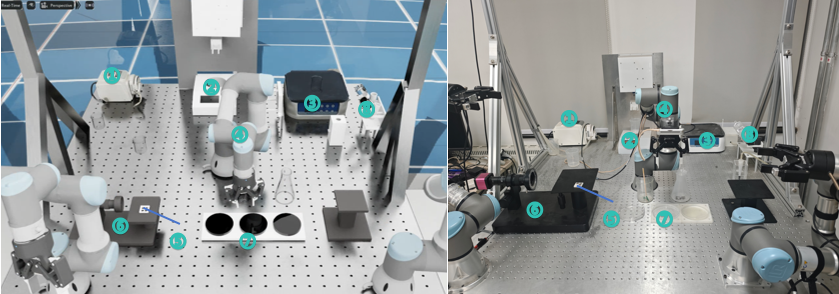
\includegraphics[width=\columnwidth]{images/sim and real.png}
    \caption{Experimental hardware platform and its simulation model in Isaac Sim, featuring the solution preparation, contact angle, and serial dilution workstations.}
    \label{fig:hardware_setup}
\end{figure}
\fi

\begin{table}[!t]
\renewcommand{\arraystretch}{1.3}
\caption{Sim-to-Real IL Success Rates for Individual Skills (not complete workflows)}
\label{tab:il_manipulation}
\centering
\resizebox{\columnwidth}{!}{%
\begin{tabular}{lcccccc}
\hline\hline
\textbf{Task} & \multicolumn{2}{c}{\textbf{Vanilla BC}} & \multicolumn{2}{c}{\textbf{DR Only}} & \multicolumn{2}{c}{\textbf{Ours (Full)}} \\ \hline
 & $n$/Succ. & Rate & $n$/Succ. & Rate & $n$/Succ. & Rate \\
Reagent Pipetting & 50\,/\,20 & 40.0\% & 50\,/\,33 & 66.0\% & 50\,/\,\textbf{42} & \textbf{84.0\%} \\
Droplet Dispensing & 50\,/\,9 & 18.0\% & 50\,/\,29 & 58.0\% & 50\,/\,\textbf{40} & \textbf{80.0\%} \\
Serial Dilution & 50\,/\,14 & 28.0\% & 50\,/\,32 & 64.0\% & 50\,/\,\textbf{42} & \textbf{84.0\%} \\ \hline
\textbf{Pooled skill trials} & 150\,/\,43 & 28.7\% & 150\,/\,94 & 62.7\% & 150\,/\,\textbf{124} & \textbf{82.7\%} \\ \hline\hline
\end{tabular}
}
\end{table}

The Wilson 95\% CIs for the pooled skill-trial rates are [22.0,36.4]\%, [54.7,70.0]\%, and [75.8,87.9]\% for Vanilla BC, DR Only, and DR + Few-Shot, respectively. These pooled denominators do not represent complete end-to-end runs and should not be used as workflow success rates. The 50-trial Wilson CIs for the proposed method are [71.5,91.7]\% for pipetting, [67.0,88.8]\% for dispensing, and [71.5,91.7]\% for dilution.

As detailed in Table \ref{tab:il_manipulation}, \textit{Vanilla BC} failed catastrophically due to the reality gap induced by transparent labware and liquid specular reflections. While DR significantly improved visual robustness, the policy still struggled with the unmodeled compliance of the physical gripper pads during multi-well alignment. Our regularized few-shot fine-tuning pipeline effectively calibrated these subtle physical discrepancies, elevating the overall success rate to 82.7\% with minimal real-world trial-and-error.

\subsubsection{Few-Shot Sample Efficiency}
\label{subsec:few_shot}

We analyzed the impact of the number of real-world demonstrations $M$ on the fine-tuning performance. Table \ref{tab:few_shot} presents the results across different $M$ values.

\begin{table}[!t]
\renewcommand{\arraystretch}{1.3}
\caption{Impact of Few-Shot Demonstration Count}
\label{tab:few_shot}
\centering
\begin{tabular}{lccc}
\hline\hline
\textbf{Demos ($M$)} & \textbf{Trials} & \textbf{Successes} & \textbf{Rate (\%)} \\ \hline
0 (DR Only) & 50 & 31 & 62.0 \\
5 & 50 & 39 & 78.0 \\
10 & 50 & \textbf{42} & \textbf{84.0} \\
20 & 50 & 42 & 84.0 \\
50 & 50 & 43 & 86.0 \\ \hline\hline
\end{tabular}
\end{table}

The existing summary gives 84.0\% success at $M=10$, but does not by itself establish an optimal demonstration budget or a statistically reliable plateau. The task identity, demonstration duration, training seeds, and relationship of this evaluation batch to Table~\ref{tab:il_manipulation} must be documented before making that claim.

For the supplementary sample-efficiency study, fix the DR-pretrained checkpoint and compare $M\in\{0,5,10,20\}$ complete real demonstrations; $M=0$ denotes the unchanged DR policy. Draw nested subsets from a training-only demonstration pool and repeat subset selection and adaptation across seeds, using the same held-out test-condition distribution for all budgets. Select hyperparameters using validation data, not test outcomes. Report precision, success with CIs, demonstration acquisition time, and adaptation time. The existing $M=50$ row is retained as a reported summary, not as a newly completed part of this supplementary study.

\subsubsection{Held-Out Conditions and Generalization}
\label{subsec:transfer_generalization}
After adaptation, freeze all policies and evaluate nominal conditions, held-out configurations within the documented DR support, and conditions outside that support separately. Use controlled changes in object starting position, illumination, and compatible container dimensions, first varying one factor at a time. Report numerical training and testing ranges and the real-demonstration coverage. A condition is outside the training support only when it is absent from both simulation randomization and real adaptation data; new samples inside the DR ranges demonstrate in-distribution robustness, not out-of-distribution transfer. Restrict physical tests to the validated hardware safety envelope.

Apply the same trial budget and task acceptance rules to each method and condition. Report absolute precision and success, changes relative to nominal conditions, and failure categories. Do not pool different conditions into a single generalization score without the condition-level results. These tests and their numerical outcomes remain pending; no generalization improvement is inferred from the current nominal success tables. In subsequent complete-workflow runs, carry the policy variant and run identifier through to film-quality measurements to examine whether improved operation performance also improves workflow reliability and accepted-film yield.

\subsection{Thin-Film Fabrication and Materials-Quality Evaluation}
\label{subsec:exp_dipcoat_quality}

% Temporarily hidden at the author's request (former Fig. 7).
\iffalse
Figure~\ref{fig:thin_film_sequence} shows robotic access to the drying oven used in the film-processing workflow.
\begin{figure*}[!t]
    \centering
    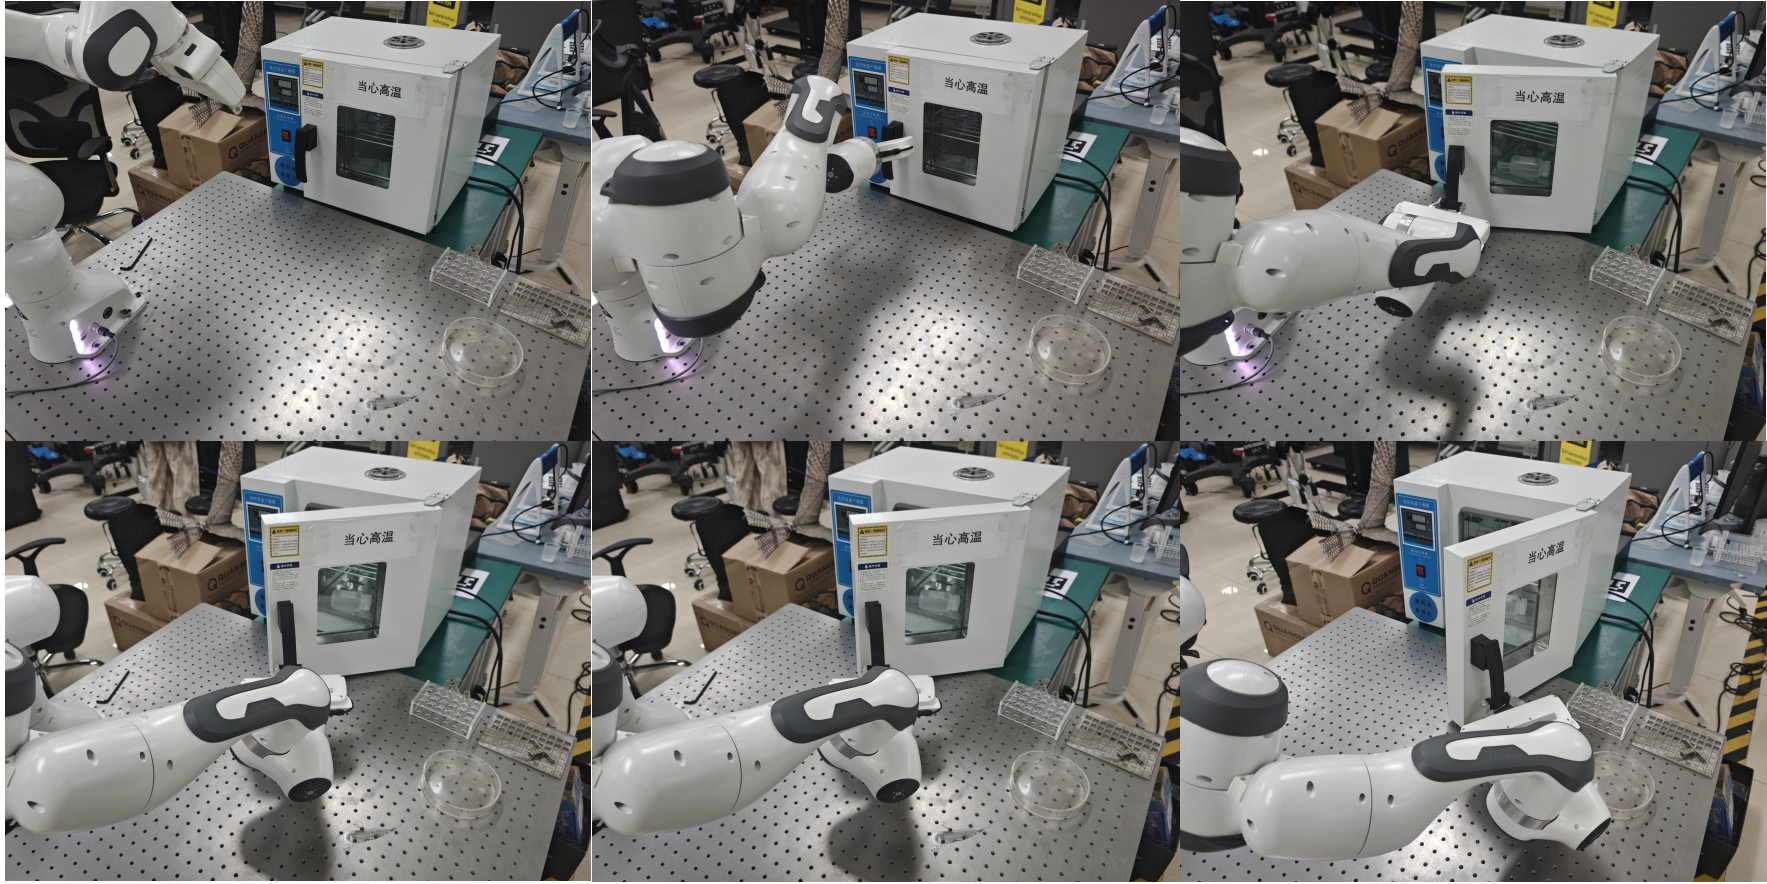
\includegraphics[width=0.9\textwidth]{images/thin_film.png}
    \caption{Robotic oven-handling sequence in the thin-film processing workflow, read from left to right across the upper row and then the lower row. The snapshots show approach, door-handle manipulation, and access to the oven.}
    \label{fig:thin_film_sequence}
\end{figure*}
\fi
The completed dip-coating experiments should be reported as a materials-quality comparison, not only as robotic motion success. We compare three execution modes under the same precursor batch, substrate preparation, immersion depth, dwell time, withdrawal-speed target, drying/curing conditions, and measurement schedule: manual dip-coating by a trained operator, a fixed robot trajectory, and the proposed learned control policy. Substrates are randomly assigned to modes, and the operator performing materials characterization is blinded to the mode where feasible. The number of independent substrates, rather than the number of measurement points on one substrate, is the statistical sample size.

Film thickness is measured at prespecified positions on each substrate. For substrate $i$, thickness uniformity is summarized by $\mathrm{CV}_{h,i}=100s(h_{ij})/\bar h_i$, with the within-substrate mean $\bar h_i$ and standard deviation $s(h_{ij})$ reported separately. Static water-contact angle is measured at multiple prespecified locations with the droplet volume and post-deposition delay held constant; report both the mean angle and spatial standard deviation. Surface roughness is reported as $R_a$ or $R_q$ from profilometry or AFM over a fixed scan area. Corrosion resistance is evaluated using the same electrolyte, exposed area, temperature, stabilization time, and electrochemical protocol for all groups; report corrosion-current density $i_{\mathrm{corr}}$ from polarization fitting and, where available, low-frequency impedance $|Z|_{0.01\,\mathrm{Hz}}$ from EIS. Coating success should be defined before analysis by explicit acceptance limits for uniformity, adhesion, and defects, not by visual inspection alone.

\begin{table*}[!t]
\renewcommand{\arraystretch}{1.2}
\caption{Thin-film quality comparison across manual, fixed-trajectory, and learned control. Replace ``pending'' with measured values; no result is inferred from robot-task success.}
\label{tab:film_quality}
\centering
\begin{tabular}{lcccccc}
\hline\hline
\textbf{Execution mode} & \textbf{Substrates $n$} & \textbf{Thickness $\bar h$} & \textbf{Thickness CV (\%)} & \textbf{Contact angle ($^\circ$)} & \textbf{Roughness $R_a$} & \textbf{$i_{\mathrm{corr}}$} \\ \hline
Manual operator & pending & pending & pending & pending & pending & pending \\
Fixed robot trajectory & pending & pending & pending & pending & pending & pending \\
Learned control (ours) & pending & pending & pending & pending & pending & pending \\ \hline\hline
\end{tabular}
\end{table*}

Report measurement units, substrate-level mean $\pm$ standard deviation, and 95\% confidence intervals in the final table. The corrosion result should additionally include $|Z|_{0.01\,\mathrm{Hz}}$ or an independently measured protection metric if available. Compare the three groups using a prespecified test appropriate to the distribution and independent-substrate design, with multiplicity correction for pairwise comparisons. The numerical film-quality results have not yet been supplied for this manuscript revision; thus no superiority or corrosion-resistance claim is made here.

\subsection{Failure-Mode Analysis}
Every failed run should receive one primary failure code based on the first unrecovered cause: perception, grasp, pipetting, docking/handover, transport/spill, communication, or recovery exhaustion. Secondary contributing codes may be retained separately. For each workflow, report the count and proportion of all failed runs in each category, the number recovered, and time lost; this avoids double-counting one run in several failure categories. The current aggregate counts do not allow this breakdown, so the analysis is pending run-level logs.

\subsection{Scientific-Outcome Acceptance and Statistical Analysis}
\label{subsec:science_quality_stats}
Robot motion completion and scientifically valid output are separate endpoints. For solution preparation, report target-versus-measured concentration error and pipetting coefficient of variation (CV) over independent preparations. For dilution, fit measured concentration against nominal dilution level and report slope, $R^2$, and per-level relative error, together with negative-control contamination rate. For thin films, use the thickness CV, contact-angle deviation, roughness, and corrosion metrics in Table~\ref{tab:film_quality}. Define acceptance thresholds before inspecting group outcomes and report the percentage of independent runs meeting every required criterion.

For key binary comparisons, report numerator, denominator, Wilson 95\% CI, and a two-sided Fisher exact test when runs are independent; use a paired exact test if methods are evaluated on matched instances. For continuous quality metrics, report effect sizes and episode- or substrate-clustered bootstrap 95\% CIs, with multiplicity correction for planned pairwise tests. Raw trial identifiers and measurements are needed to calculate valid $p$-values and clustered intervals; none are invented from the summary tables.

\subsection{End-to-End Autonomous Workflow Integration}
\label{subsec:exp_end_to_end}

To isolate the effect of failure-aware orchestration, a dedicated comparison should run the same low-level skills under (i) a fixed sequential state machine that terminates on any failed guard and (ii) the proposed HSM with bounded recovery. Both variants should use identical initial conditions and injected failures, including missed grasps, docking offsets, and stale perception. Report the number of trials, full-workflow success, stage-specific failure and recovery rates, number of retries, operator interventions, and completion time. The results below do not include this ablation, so they should not be interpreted as evidence that the HSM outperforms fixed sequencing.

Complete-workflow success must be defined on a single, preregistered sequence of operations, with the same run ID carried through every stage and no denominator reset after failure. We distinguish (i) solution preparation: reagent acquisition, dosing, mixing, and quality check; (ii) thin-film fabrication: solution delivery, substrate preparation, dip-coating, curing, and film-quality acceptance; and (iii) serial dilution: reagent delivery, tip handling, dilution, and concentration/contamination acceptance. A run succeeds only if all required stages and scientific-quality thresholds pass without unplanned human intervention. Record retries and recovery separately, and report both first-pass and recovery-assisted success.

The existing stage-level counts below were collected for individual operations and cannot be multiplied, pooled, or interpreted as complete-workflow outcomes. In particular, the previously reported ``42/50 full-loop'' value is inconsistent with the 40/50 contact-angle stage count if both describe the same 50 runs; the underlying run-level log must be reconciled before reporting an end-to-end rate. The statement about ten consecutive successful cycles likewise requires identifiable run records and is not treated as an independently verified result here.

\begin{table}[!t]
\renewcommand{\arraystretch}{1.3}
\caption{Existing Stage-Level Counts; Full-Workflow Outcomes Require Run-Level Logs}
\label{tab:end_to_end}
\centering
\begin{tabular}{lccc}
\hline\hline
\textbf{Workflow Stage} & \textbf{Trials} & \textbf{Successes} & \textbf{Rate (\%)} \\ \hline
Autonomous Transit & 50 & 44 & 88.0 \\
Upright Grasping & 50 & 43 & 86.0 \\
Reagent Pipetting & 50 & 42 & 84.0 \\
Contact Angle Measurement & 50 & 40 & 80.0 \\
Serial Dilution & 50 & 42 & 84.0 \\ \hline
\textbf{Complete workflow} & \textbf{pending} & \textbf{pending} & \textbf{pending} \\ \hline\hline
\end{tabular}
\end{table}

\begin{table}[!t]
\caption{Complete-Workflow Reporting Template (independent runs)}
\label{tab:workflow_complete}
\centering
\begin{tabular}{lccc}
\hline\hline
\textbf{Workflow} & \textbf{Runs} & \textbf{First-pass} & \textbf{With recovery} \\ \hline
Solution preparation & pending & pending & pending \\
Thin-film fabrication & pending & pending & pending \\
Serial dilution & pending & pending & pending \\ \hline\hline
\end{tabular}
\end{table}

% \begin{figure*}[!t]
%     \centering
%     % \includegraphics[width=\textwidth]{figures/end_to_end_snapshots.png}
%     \caption{Sequential snapshots of the autonomous three-stage laboratory workflow: (a)--(b) Upright labware grasping and reagent pipetting; (c)--(d) Constraint-aware transit and droplet dispensing for water contact angle detection; (e)--(f) High-precision serial dilution and microplate alignment.}
%     \label{fig:sequential_snapshots}
% \end{figure*}
